\documentclass[11pt]{article}
\usepackage{acl2010}
\usepackage{times}
\usepackage{url}
\usepackage{latexsym}
\usepackage{graphicx}
%\setlength\titlebox{6.5cm}    
% You can expand the title box if you really have to

\newcommand{\mnote}[1]{\marginpar{%
  \vskip-\baselineskip
  \raggedright\footnotesize
  \itshape\hrule\smallskip\tiny{#1}\par\smallskip\hrule}}  

\title{Learning Structural and Sentential Paraphrases from Parallel Corpora}

\author{Juri Ganitkevitch \and Chris Callison-Burch\\ 
Center for Language and Speech Processing\\ 
Johns Hopkins University}

\date{}

\begin{document}
\maketitle

\begin{abstract}
Damn it feels good to be a gangsta.
A real gangsta-ass nigga plays his cards right.
A real gangsta-ass nigga never runs his fuckin mouth.
'cause real gangsta-ass niggas don't start fights.
And niggas always gotta high cap.
Showin' all his boys how he shot em.
But real gangsta-ass niggas don't flex nuts.
'cause real gangsta-ass niggas know they got em.
And everythings cool in the mind of a gangsta.
'cause gangsta-ass niggas think deep.
Up three-sixty-five a year 24/7.
'cause real gangsta ass niggas don't sleep.
\end{abstract}

\section{Introduction} \label{introduction}

Paraphrases are alternative ways to express the same meaning. The
automated generation and detection of paraphrases is crucial to many
tasks in NLP and has been shown to improve performance in others. In
multi-document summarization systems, paraphrase detection can be used
to recognize and collapse redundancies \cite{Barzilay1999}. Used for
query expansion, paraphrasing improves the performance of question
answering \cite{Ravichandran2002,Riezler2007} and information
retrieval systems \cite{Anick1999}. In machine translation,
paraphrases have been used to extend phrase tables in order to achieve
broader source language coverage \cite{Callison-Burch2006b}, as well
as to automatically generate additional reference translations,
leading to better results in minimum error rate training
\cite{Madnani2007}.

The notion of a paraphrase typically denotes a set of surface text
forms with the same meaning:
\begin{center}
\begin{tabular}{c}
the committee's proposal \\
the proposal of the committee
\end{tabular}
\end{center}
Introducing non-terminals or \emph{slots}, lexical paraphrases are
commonly generalized into paraphrase patterns such as:
\begin{center}
\begin{tabular}{c}
the $X_1$'s $X_2$ \\
the $X_2$ of the $X_1$
\end{tabular}
\end{center}
It is evident that, compared to plain phrases, paraphrase patterns
have a much higher potential at generalization. However, the
unconstrained nature of the slots also bears the risk of producing
nonsensical or ungrammatical output. Thus, in order to achieve more
well-formed results, the slots are typically augmented with syntactic
constraints, yielding syntactic paraphrases.
\begin{center}
\begin{tabular}{c}
the $NP_1$'s $NP_2$ \\
the $NP_2$ of the $NP_1$
\end{tabular}
\end{center}
While retaining the generalization capabilities of unconstrained
patterns, the application of syntactic paraphrases is more controlled
and yields higher quality output.

\mnote{Sentential paraphrases, and all the transforms we want to
  learn. Unclear whether we can get them from bitexts.. ..let's find out.}

In this paper, we demonstrate the integration of syntactic paraphrases
into a machine translation-based paraphrasing system. The use of MT
machinery and models to extract and apply paraphrases from bilingual
parallel corpora by pivoting over foreign language phrases is a
well-known technique. \newcite{Zhao2008b} have presented results that
indicate that bilingually sourced paraphrase extraction significantly
outperforms monolingual approaches in both recall and
precision. However, while in monolingually sourced paraphrase
extraction linguistically informed paraphrase patterns are
commonplace, MT-based paraphrase systems mostly have been limited to
lexical paraphrases \cite{Quirk2004,Callison-Burch2005} or
unconstrained patterns \cite{Madnani2007}. In recent efforts to enrich
pivot-based paraphrase extraction with linguistic information
\newcite{Callison-Burch2008} showed that enforcing syntactic
constraints can drastically improve the quality of a lexical
paraphrase system. \newcite{Zhao2008} used dependency parses on the
English side of a large bilingual corpus to produce syntactic
parapharse patterns. Our approach goes beyond these two and produces a
fully syntactically informed synchronous paraphrasing CFG.

An additional focus of this paper are the closely tied topics of model
parameter estimation and system evaluation. In practice, the nature of
paraphrasing as a component of larger systems makes meaningful
standalone evaluation difficult: in many applications of paraphrasing
the proper preservation of meaning and production of grammatical
output is only a basis requirement. Additional constraints imposed by
the task at hand, be it shortening the input for sentence compression
or generating significantly differing output for the generation of
additional references, are a crucially important factor for the
system's quality. However, this is often not reflected when estimating
the parameters of a paraphrasing system. We leverage the rich feature
set present in our approach and the flexibily of minimum error rate
training to specifically adapt our paraphrase system to the task of
reference expansion for MT and demonstrate how it outperforms the
commonly used approach.

This paper is structured as follows: we present related work on
paraphrase acquisition in
Section~\ref{related_work}. Section~\ref{formalism} introduces the
machine translation formalism used in our work. In
Section~\ref{acquisition} we describe our paraphrase acquisition
approach. Sections~\ref{adaptation} and \ref{analysis} present our
parametere estimation setup, experimental and an analysis
thereof. Finally, we conclude in Section~\ref{conclusion}.

\section{Related Work} \label{related_work}

The paraphrase extraction task has received a fair amount of attention
in the past. The bitext-based pivot approach we build on in this paper
was first introduced by \newcite{Callison-Burch2005}. They use the
well-established MT pipeline \mnote{Cite MT papers?} to word-align a
parallel bitext and extract a bilingual phrase table. This table
contains phrase pairs $(e, f)$ (where the $e$ and $f$ stand for
English and foreign phrases, respectively) as well as bi-directional
translation probabilities $p(f | e)$ and $p(e | f)$, computed from the
relative frequencies of $e$ and $f$. From this table, they compute a
paraphrasing phrase table with entries $(e, e')$ and a paraphrase
probability
\begin{equation}
p(e | e') = \sum_f p(e | f) p(f | e') .
\end{equation}
Additionally, the resulting paraphrases are further re-ranked using
contextual features such as a language
model. \newcite{Callison-Burch2008} improves on this method by
requiring the paraphrases to be governed by the same constituent,
resulting in less noisy and more grammatical paraphrases.

\newcite{Madnani2007} apply the pivot technique to the synchronous CFG
formalism intoduced by \newcite{Chiang2005}, taking the step from a
paraphrase table to a grammar of paraphrase rules, corresponding to
the slotted patterns introduced above. Following the widely used MT
pipeline setup, their paraphrasing system employs the familiar
log-linear model with a featureset that mirrors those in classic MT
systems. The parameters for the log-linear model are estimated using
minimum error rate training, maximizing the BLEU metric on a set of
parallel English sentences. The authors report significant gains in
translation quality when using additional references generated by
paraphrasing to tune an MT system.

Enriching pivot-based paraphrase extraction with syntactic
information, \newcite{Zhao2008} extract partial subtrees from the
dependency-parsed English side of a bitext and pivot over the
corresponding Chinese phrases to align them to paraphrases. The slots
in the resulting patterns are labeled with part-of-speech tags. Their
system employs a log-linear model that combines translation and
lexical probabilities and is tuned to maximize precision over a
hand-labeled set of paraphrases.

Several research efforts have leveraged parallel monolingual corpora,
however they jointly suffer from the scarcity and noisiness parallel
corpora. \newcite{Dolan2004} \mnote{Cite \cite{Dolan2005}, too.} work
around this issue by extracting parallel sentences from the vast
amount of freely available comparable English text and apply machine
translation techniques to create a paraphrasing system
\cite{Quirk2004}. However, the word-based translation model and
monotone decoder they use results in a substantial amount of identity
paraphrases or single-word substitutions.

Relying on small data sets of semantically equivalent translations,
\newcite{Pang2003} created finite state automata by syntax-aligning
parallel sentences, enabling the generation of additional reference
translations.

Both \newcite{Barzilay2001} and \newcite{Ibrahim2003} sentence-align
existing noisy parallel monolingual corpora such as translations of
the same novels. While \newcite{Ibrahim2003} employ a set of
heuristics that rely on anchor words identified by textual identity or
matchin liguistic features such as gender, number or semantic class,
\newcite{Barzilay2001} use a co-training approach that leverages
context similarity to identify viable paraphrases.

Semantic parallelism is well-established as a stong basis for the
extraction of correspondencies such as paraphrases. However, there are
notable efforts that choose to forgo it in favor of clustering
approaches based on distributional characteristics. The well-known
DIRT method by \newcite{Lin2001} fully relies on distributional
similarity features for paraphrase extraction. Patterns extracted from
paths in dependency graphs are clustered based on the similarity of
the observed contents of their slots.

Similarly, \newcite{Bhagat2008} argue that vast amounts of text can be
leveraged to make up for the relative weakness of distributional
features compared to parallelism. They also forgo complex annotations
such as syntactic or dependency parses, relying only on part-of-speech
tags to inform their approach. In their work, relations are learned by
finding pattern clusters initially seeded by already known
patterns. However, this method is not capable of producing syntactic
paraphrases. \mnote{Need better tie-in with the overall theme of structural
paraphrases.}




\section{The SAMT Formalism} \label{formalism}

The \emph{Syntax Augmented Machine Translation} (SAMT,
\cite{Zollmann2006})


\section{Paraphrase Acquisition} \label{acquisition}

\begin{figure}
\begin{center}
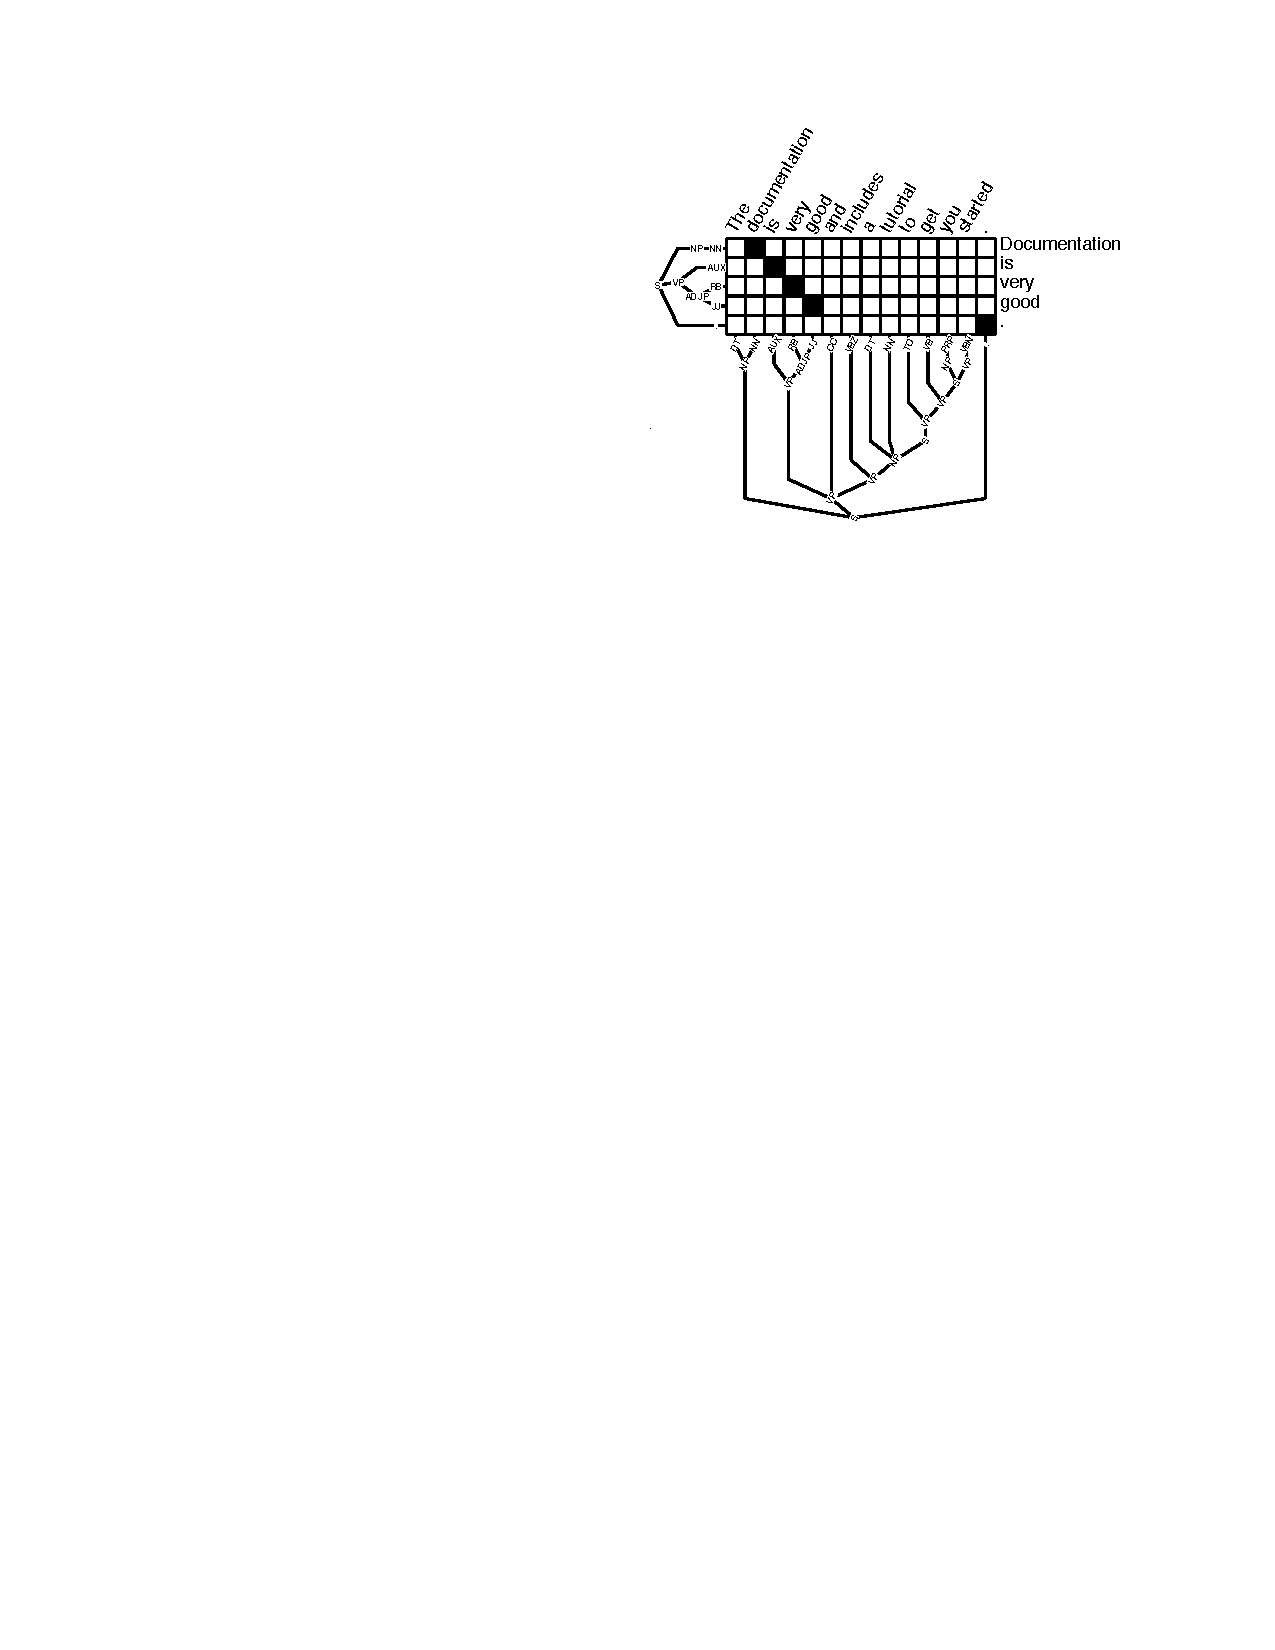
\includegraphics[width=0.99\linewidth]{figures/tree_placeholder.pdf}
\end{center}
\caption{A figure I stole from Trevor \& Mirella}
\end{figure}


Formal: Synchronous grammars, with the usual examples (one phrasal, one
structural).

Formal: Log-linear model for features, weights will be optimized to some
objective, we discuss those in later section.

Diagram for grammar extraction (two sentence pairs with trees and
alignments, show how that gets us a paraphrase pattern). 



\subsection{Paraphrase Grammar Extraction} \label{extraction}

Some talk about the SAMT approach needs to go here. 

We extract SAMT translation grammars for nine languages. Give some
details on the pipeline, mention that the grammars are
\emph{gargantuan} (this word needs to be in the paper!), but that the
whole process is very well-suited for MapReduce (even though, we
didn't use it).

\subsection{Creating Paraphrase Rules} \label{rule_creation}

\subsubsection{Rule Body} \label{rule_body}

To create paraphrase rules from bilingual translation rules, we pivot
over the foreign side of the translation rule, with the additional
constraint that the rule's head, i.e.\ the label that governs the
rule.

Mention the proper mapping and flipping of nonterminals.

\subsubsection{Rule Features} \label{rule_features}

The SAMT grammars our paraphrasing system is based on provide a rich
feature set that takes into account source- and target-side
frequencies, reordering of NTs and lexical translation probablities
for each rule. When transforming the bilingual grammars into a
monolingual paraphrase grammar we preseve the feature set and

Shouldn't give details on every single feature, but point out some key
approaches:
\begin{itemize}
\item probablistic features multiply 
\item target-side indicator features are inherited
\item actually state what happens with other indicator features
  (re-ordering, punctuation, rareness etc)
\end{itemize}


\section{Task-Specific Parameter Estimation} 
\label{adaptation}

have to estimate parameters now

general approach: decide on an objective function, choose parameters
such that

Having extracted a paraphrase grammar, we are left with the task of
estimating the parameters $\lambda_i$ of the log-linear
model. Generally, the $\lambda_i$ are chosen to maximize a given
objective function. Ideally, the objective function mimics the
system's intended use, so that parameter estimation tunes the system
to optimal practical performance.

Many previously proposed paraphrase extraction methods focus on
maximizing recall and precision over a manually annotated set of
paraphrase patterns \cite{Zhao2008,Bhagat2008}.  Similarly, paraphrase
approaches that utilize machine translation machinery do not stray
from the usual pipeline, using MERT \cite{Och2003} to tune the
paraphrase system to produce good English output by maximizing BLEU
score on a set of known paraphrases \cite{Madnani2007}.

While these methods may produce well-weighted collections of
paraphrase patterns, they do not emphasize 

it results in a paraphrase system that is not
focussed on any particular task.



\subsection{Reference Expansion}

We present an examplary application of our paraphrasing system

Using paraphrases for reference expansion, cite Madnani

idea behind reference expansion: create additional ``reference''
translations to tune a machine translation system

however, tuning our paraphrase system to BLEU results in a paraphraser
that generates only minimal changes \mnote{if so, how did Madnani deal
with that?}

We therefore implement a paraphrase-specific metric, ppBLEU, that aims
to amend this issue.

\subsubsection{Paraphrase BLEU} \label{pp_bleu}

the familiar BLEU metric (cite BLEU) quantifies the quality of a
translation by measuring the n-gram overlap between the generated
translation and a set of  reference translation

for paraphrasing, this can be a problem, since the reference
translations typically have a rather high overlap with one another
\mnote{get some numbers to back that up}


\subsubsection{Data} \label{data}

We use Europarl v. 5. Align with Berkeley and parse with The Parser.

we use the SAMT pipeline to extract the grammar

however, the pivoting approach makes it impossible to apply the common pre-emptive
grammar filtering, hence the grammar grows very large

\subsubsection{Evaluation} \label{evaluation}

A straightforward way to evaluate a paraphrasing system is by using to
improve an SMT system's performance. Cite Chris and Nitin. Compare to
Hiero baseline.



\section{Analysis} \label{analysis}

There are two main motivations to impose syntactic contraints on
paraphrase patterns: firstly, we aim for an increase in paraphrase
quality. I.e.\ we expect our training procedure to learn properly
labeled patterns that properly reflect well-know paraphrastic
transformations such as passivization, dative shift or the possessive
rule. Secondly, we hope to find structural paraphrases that capture
long-distance reorderings, leading to sentential paraphrases.

\subsection{Comparison of Paraphrase
  Patterns} \label{pattern_comparison}

To analyze the paraphrase patterns produced by our system, we reduce
the grammar to only patterns that apply to an example sentence and
take a closer look at the most likely pattern pairs. We contrast our
extracted paraphrases with a Hiero-style baseline that mirrors the
approach of \newcite{Madnani2007}. 

\begin{table*}[ht]
\begin{center}
\begin{tabular}{|c|c|c|c|}
  \hline
  \multicolumn{2}{|c|}{Hiero baseline} & \multicolumn{2}{c|}{SAMT
    paraphrase} \\
  \hline
  blah & blah & blah & blah \\
  blah & blah & blah & blah \\
  blah & blah & blah & blah \\
  blah & blah & blah & blah \\
  \hline
\end{tabular}
\end{center}
\caption{This table shows some example paraphrases}
\end{table*}


\subsection{Sentential Paraphrasing} \label{sentential_paraphrasing}

We are interested in sentential paraphrases. Why are we interested?
More powerful than locally constrained, gives us large-scale changes
to sentential structure, which can be cruicial to applications such as
detecting entailment or automatically creating significantly differing
references. \emph{However, phrasal decoder-based approaches should be
  able to achieve similar re-ordering effects (if not the generality,
  which we only implicitely achieve, really). Maybe we should add a
  phrase-based baseline in addition to Hiero? Did Nitin talk about
  this?}

While the definition of a phrasal paraphrase is intuitively clear,
sentential paraphrases are much harder to define. When paraphrasing a
sentence $s$ into a new sentence $t$, the term suggests that we expect
the changes to $s$ to be above a certain threshold for $t$ to be
considered a sentential paraphrase. 

\section{Conclusion} \label{conclusion}

Look, we unified everything in the field and made all this stuff from
the previous section much better. Or did we?

\bibliographystyle{acl}
\bibliography{paraphrasing}

\nocite{*}

\end{document}

